he \h\ abundance depends on several factors: the abundance of H, the
abundance of free electrons (ionized from other species present in the
atmosphere, including H), and the factors that lead to the conversion
of \h\ back to H: photoionization and collisions with other particles.  All
of these factors have some sort of dependence on temperature.

%The solar atmosphere is made up about 70\% by mass of H.  As will be
%shown in what follows, the fraction of H atoms that are taken up in
%\h\ is small, and as is shown in section 7.4 of \cite{boehm1989} the
%fraction of H atoms

%Because the creation of \h\ depends not only on the normal Saha
%equation calculation of relative abundances (in our case,
%$N(H)/N(H^-)$) but also on the presence of free electrons the normal
%Saha equation can be written in the form (\citealt{collins1989})
%\beq
%\label{eq:saha}
%\frac{N(H)}{N(H^-)} = \Phi (T) P_e
%\eeq
%where $P_e$ is the electron pressure (and is hence dependent on the
%ionization states of all species present in the solar atmosphere) and
%$\Phi (T)$ is the normal partion functional form of the Saha
%ionization equation

The abundance of an ionized species can be calculated using the Saha
ionization equation, which is given by
\beq
\label{eq:saha}
\frac{N(X_{i+1})}{N(X_{i})} = \frac{(2\pi m k T)^{1.5}}{n_e h^3}\frac{2g_{i+1}}{g_{i}}e^{-\chi/kT}
\eeq
 where $\chi$ is the energy difference between the two ionization
states, $n_e$ is the number density of electrons, $k$ is the Boltzmann
constant, $h$ is the Planck constant, $T$ is the temperature, $X_i$ is
an atom $X$ in the $i$th ionization state, and $g_i$ is the degeneracy
factor corresponding to the $i$th ionization state.  Specifically
for \h\ we get
\beq
\label{eq:thisone}
\frac{N(H)}{N(H^-)} = \frac{(2\pi m k T)^{1.5}}{n_e h^3}2\frac{1}{2}e^{-0.754\textrm{eV}/kT}.
\eeq
In practice using equation~\ref{eq:saha} is complicated by the fact that
$n_e$ is determined by electrons contributed from all species, not
just the specific atom/ion in question.  It can be calculated by
summing over the number density
of ionized particles multiplied by their degree of ionization (whether
they contribute one electron, two electrons, etc.). This is expressed by
\beq
\label{ref:ne}
n_e = \sum\limits_{X,i}i\times n_{Xi}
\eeq
where $X$ again represents a specific atom and $i$ represents the ionization state
of the atom, thus summing over all possible ions of all atoms.  Since,
as can be seen in equation~\ref{eq:saha} $n_{ij}$ also depends on
$n_e$ we end up with a system of equations that, when rounded out with
equation~\ref{ref:ne}, gives us the same number of equations and
unknowns.  However, values for $n_e$ in the sun have been previously
calculated. I will use the value given in \cite{boehm1989}, as
outlined later on.  

The relative contributions of the elements to the overall electron
density can be calculated without actually knowing the electron
density.  If we know the abundance of an element relative to H we can
define a relative contribution factor $R$ by 
multiplying the abundance by the ionization ratio given in the Saha
equation,
\beq
R_i \equiv B \frac{N(X_{i+1})}{N(X_{i})} \frac{N(X_{i})}{N(H)}
\eeq
where $B$ is a normalization constant.

Table~\ref{tab:electroncontribution} shows the abundance, ionization
potential (abbreviated as ``I.P.''), and relative contribution factor $R$ for the species with
the largest contributions to $n_e$ in the solar atmosphere, in order
of increasing atomic number.
Abundances are taken
from \cite{grevesse1998}\footnote{\cite{grevesse1998} did not have an
abundance quoted for Cs, which, with its low ionization potential of
3.894 eV would make a significant contribution to $n_e$ even in low
abundances. \cite{grevesse1998} did not make it clear whether the
omission was due to lack of measurements or lack of Cs.  Since Cs has
one stable isotope, $^{133}$Cs, we cannot conclude its lack in the
solar atmosphere from radioactive decay alone.}   and are in the form $A_j
= \log N(j)/N(H) + 12.0$ where $j$ represents a specific element.
Ionization potentials are taken from \cite{moore1970} and represent
the ionization potentials for {\it first} ionizations only, since
subsequent ionizations have large enough ionization potentials as to
render their contributions to the overall $n_e$ negligible.  $R$ is
normalized so that, for Na (the atom with the lowest atomic number
that makes a significant contribution) $R=1.0$.  Except for H, only
atoms with $R>0.01$ are included in
table~\ref{tab:electroncontribution}.  Other atoms have
too low of abundances and/or too high of ionization potentials to have a
significant contribution to $n_e$.
\begin{table}[h]
\caption{\label{tab:electroncontribution}Data on Atoms with Largest Contributions to Free Electron Count}
\begin{tabular}{c c c c}
Atom & Relative Abundance $A_j$ & I.P. (eV)& $R$\\
H & 12.0 & 13.598 & $\sim$10$^{-5}$\\
%Li & 1.10 & 5.392 & 0.0032\\
Na & 6.33 & 5.139 & 1.0 \\
Mg & 8.151 & 7.046 & 0.54\\
Al & 6.47 & 5.986 & 0.070\\
K  & 5.12 & 4.341 & 1.5\\
Ca & 6.36 & 6.113 & 0.58\\
Rb & 2.60 & 4.177 & 0.17\\
Sr & 2.97 & 5.695 & 0.045\\
Ba & 2.13 & 5.212 & 0.052\\
\end{tabular}
\end{table}

The largest contributions to $n_e$ are made by the alkali metals Na
and K, followed by their same period alkaline earth metal counterparts,
Mg and Ca  (Li and Be have abundances much too low to make
significant contributions to $n_e$).  Rb, the next period alkali
metal, is next in contribution importance, followed by Al, Ba, and
Sr.  Thus, the alkali and alkaline earth metals, with their small
ionization potentials and (in the case of the period 3 and 4 elements)
large abundances, dominate the contributions to $n_e$.  H, the most
abundant atom in the solar atmosphere, only has a contribution
relative to that of Na of one part in $10^5$.  He has a contribution
relative to that of Na of one part in $10^{15}$.  Thus the presence of
alkali and alkaline earth metals in the solar atmosphere provide a
vital contribution to $n_e$ that H and He by themselves cannot make,
which in turn affects the \h\ abundance and its contribution to the
opacity.  This is seen in figure~\ref{fig:l}, where the metal-free
population III stars have a lower opacity for $T\lesssim 5\times 10
^{3} K$.
\begin{figure}
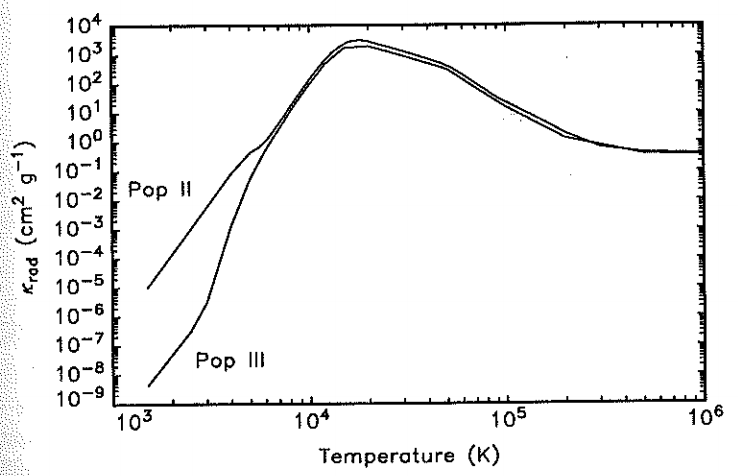
\includegraphics[width=\linewidth]{figs/opacitysee.png}
\caption{\label{fig:l}From \cite{hansen1994stellar}.  ``Pop II'' has
metallicity $Z=0.02$, while ``Pop III'' has no metals.  The density is
$10^{-6}$ g cm$^{-3}$.}
\end{figure}


\cite{boehm1989} actually cites the electron abundance in terms of the electron
pressure, $P_e=n_e kT$. She
expresses the Saha equation in the logarithmic form
%\begin{align}
\begin{multline}
\log \frac{N(X_{i+1})}{N(X_i)} = \log \frac{u_{i+1}}{u_i}+\log 2 +\\
 2.5 \log T - \chi \theta - \log P_e - 0.48
\end{multline}
%\end{align}
where log is log$_{10}$, $\theta$ is a temperature parameter given by
$\theta = 5040/T$ ($T$ is in Kelvin), and $u$ is the partition function
\beq
u_i = g_i + \sum\limits_{n=2}^{\infty} g_{in} e^{\chi_{in}/kT}
\eeq
which is summed over all the energy levels of a particular species.
Using the value given in \cite{boehm1989} for the electron pressure in
the solar photosphere 
($\log P_e = 1.5$) we can calculate the abundance of \h\ relative to H
(using 5778 K\footnote{From NASA: www.nssdc.gsfc.nasa.gov/planetary/factsheet/ sunfact.html} as $T$)
\begin{multline}
\log \frac{N(H)}{N(H^-)} = \log \frac{4}{1} + \log 2 + 9.40 - 0.658  -
1.5 - 0.48\\ = 7.7
\end{multline}
Inverting we find 
\beq
\label{eq:hminusab}
\frac{N(H^-)}{N(H)}=10^{-7.7} \approxeq 2 \times 10^{-8}.
\eeq
There is only a small fraction of H at any given time in the
photosphere that has become \h.  To understand better why \h\ in such
small abundances has such a large impact on the opacity in visible
wavelengths we must compare its abundance to other species that have
continuum opacities at visible wavelengths.  The Paschen continuum of
hydrogen (ionization from $n=3$) is the only other thing that can contribute
to continuum opacity in the visual spectral range
(\citealt{boehm1989}).  
%\cite{boehm1989} then calculates the relative
%abundances of H($n=e$) to \h\ and finds
We can calculate the relative abundance of H($n=3$) to \h.
\beq
 \frac{N(H_{n=3})}{N(H^-)} = \frac{N(H_{n=3})}{N(H_{n=1})}\frac{N(H_{n=1})}{N(H^-)}
\eeq
We can make the approximation that $N(H_{n=1})\approxeq N(H)$ since (as will be shown over the course of the next several equations) the number of H atoms with electrons in an excited state is small.
\beq
 \frac{N(H_{n=3})}{N(H^-)} = \frac{N(H_{n=3})}{N(H_{n=1})}\frac{N(H)}{N(H^-)}
\eeq
\cite{boehm1989} calculates the number of H atoms with electrons excited to $n=3$ relative to H atoms in the ground state and gets
\beq
\frac{N(H_{n=3})}{N(H_{n=1})} \approxeq 6 \times 10 ^{-10}.
\eeq
For consistency the value calculated by \cite{boehm1989} for
$N(H)/N(H^-)$ will be used, since she used a slightly different temperature than I did in my calculation (equation~\ref{eq:hminusab}) for consistency.  She calculated $N(H)/N(H^-) \approx 3 \times 10^{-8}$.  Plugging in the values we get
\beq
\frac{N(H_{n=3})}{N(H^-)} \approxeq \frac{6 \times 10 ^{-10}}{3 \times 10^{-8}} = 2 \times 10^{-2}.
\eeq
So, there is about 100 times more \h\ than hydrogen atoms at $n=3$;
assuming that the absorption coefficients of \h\ and  hydrogen atoms
at $n=3$ are within a factor of 10 it can be clearly seen from this
calculation alone that \h\ will be the dominating contribution to the
opacity at visual wavelengths.

%The Balmer continuum is in UV
\cite{boehm1989} also shows that \h\ is only about 10 times less abundant than hydrogen atoms in $n=2$.  Since the Balmer ionization energy (corresponding to photon wavelength of 3647 \AA) occurs in the ultraviolet, where \h\ contributions to opacity are less than in the optical, and there is a relatively large fraction of H$_{n=2}$ relative to \h\ there is a measurable increase in continuum opacity due to H$_{n=2}$.  %Indeed, figure~\ref{fig:bohmopacity} shows the Balmer discontinuity in the ultraviolet.

